\documentclass{ctexart}
\usepackage{listings}
\usepackage{geometry}
\geometry{a4paper,left=3cm,right=3cm,top=4.5cm,bottom=4.5cm}

\lstset{ %
    basicstyle=\footnotesize\ttfamily,        % size of fonts used for the code
    columns=fullflexible,
    breaklines=true,                 % automatic line breaking only at whitespace
    captionpos=b,                    % sets the caption-position to bottom
    tabsize=4,
    commentstyle=\color{green},    % comment style
    escapeinside={\%*}{*)},          % if you want to add LaTeX within your code
    keywordstyle=\color{blue},       % keyword style
    stringstyle=\color{mauve}\ttfamily,     % string literal style
    frame=single,
    rulesepcolor=\color{red!20!green!20!blue!20},
    % identifierstyle=\color{red},
    language={C++},
    numbers=left,
    numberstyle=\tiny,
}

\author{SOL}
\title{作业? 汇编器}

\begin{document}

\maketitle
\setcounter{page}{1}

\newpage

\section {MIPS指令}

    \subsection {机器码}
    
        \par 机器码是实际在存储器中保存的指令序列,可以被计算机直接解析执行。MIPS指令机器码拥有较为统一的格式,所以非常方便解析。
        \par 常见的MIPS机器码格式包括:
        
        \begin{itemize}
            \item CCCCCC SSSSS TTTTT DDDDD LLLLL TTTTTT (三地址,多用于R类)
            \item CCCCCC SSSSS TTTTT IIIIIIIIIIIIIIII (双地址带立即数,多用于L类)
            \item CCCCCC AAAAAAAAAAAAAAAAAAAAAAAAAA (单地址,多用于跳转)
        \end{itemize}
        \par 其中C为指令类型,S、T、D为寄存器号,A为地址,L为移位量,T为R类指令行为,I为立即数。

    \subsection {汇编指令}
        
        \par 汇编指令是机器码的另一种方便人类读写的形式,可以分为真指令和伪指令;其中一条真指令与一条机器码指令完全对应,而一条伪指令可能包含了多条机器码。
        

\section {MIPS环境模拟器}
            
    \subsection {汇编器}

        \par 将汇编指令翻译成机器码。输入指令类型,再依次解读后续参数,通过位运算写入字中。
        \par 以LW指令为例:
        
\begin{lstlisting}
    if(t == "lw")
    {
        flow >> ss >> sd;
        if(notID(ss) || notOf(sd))
            return ret;

        auto x = getOf(sd);
        res = 0; 
        setVal(res, 31, 26, LW);
        setVal(res, 25, 21, getID(ss));
        setVal(res, 20, 16, x.first);
        setVal(res, 15, 0, x.second);
        ret.push_back(res);
    }
\end{lstlisting}

    \subsection {反汇编器}
    
        \par 将机器码反汇编为汇编指令。甚至更加简单:先从高六位解析指令类型,之后将低位按照对应格式摘出即可。
        \par 同样以LW指令为例:
        
\begin{lstlisting}
    res << "lw " << getVal(s, 25, 21) << " " << getVal(s, 15, 0) << "(" << getVal(s, 20, 16) << ")";
\end{lstlisting}
        
    \subsection {模拟器}
        \par 模拟器基本上虚拟了一个简易的MIPS环境。它可以模拟内存,并且支持写入、输出数据和指令的操作。另外它可以将汇编码加载到内存,并且顺序执行,直到发现一个停止字(0xFFFFFFFF)。
        
    \subsection {更新}
    
        \begin{itemize}
\item 修正了lw和sw指令中寄存器顺序弄反的问题
\item 增加了斐波那契程序fibo.aca,可以测试循环程序
\item 更新了指令集   
\item 模拟器加入了可以查看内存二进制码的功能(原来只能看10进制并不方便)  
\item 现在可以通过寄存器名字(而不只能寄存器号)来访问一个寄存器了  
\item 进一步增加程序的稳定性,修复了会不停输出“错误的指令”的bug  
\item 对错误指令的审核更加严格,尽可能避免任何不符合格式的指令被执行  
\item 现在Mips汇编指令中必须要加入逗号,更加标准了  
        \end{itemize}

\section{测试}

    \par README文件包含使用说明。
    
\begin{figure}[htb]
	\center{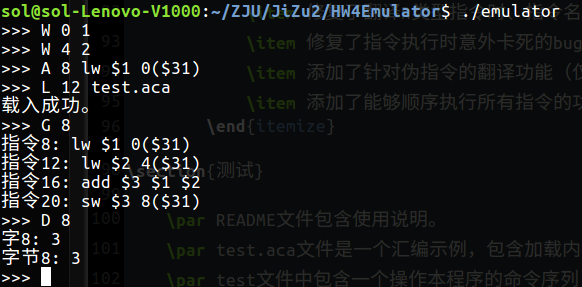
\includegraphics[scale=0.5]{res1.png}}
\end{figure}
    
\end{document}
    
    
    
    
    
    
    
    
    
